\documentclass[xcolor=dvipsnames,notes]{beamer}
\usecolortheme[named=Brown]{structure}
\usetheme{default}
\setbeamertemplate{navigation symbols}{} 
\usepackage{tikz}
\usetikzlibrary{arrows,decorations.pathmorphing,backgrounds,positioning,fit}
\usetikzlibrary{datavisualization.formats.functions}
\usetikzlibrary{shapes}
%     
%Here are some macro's saving time and labour:     
%     
\newcommand{\const}{\mbox{const}}      
\newcommand{\est}{\mbox{{\tiny est}}}      
\newcommand{\im}{\mbox{$\Im \mbox{m}$}}      
\newcommand{\obs}{\mbox{{\tiny obs}}}      
\newcommand{\otherwise}{\mbox{otherwise}}      
\newcommand{\real}{\mbox{$\Re \mbox{e}$}}      
\newcommand{\sign}{\mbox{sign}}      
\newcommand{\sinc}{\mbox{sinc}}      
%
\newcommand{\p}{\mbox{$\partial$}}      
\renewcommand{\d}{\mbox{$\partial$}}      
\newcommand{\w}{\mbox{$\omega$}}      
%
\newcommand{\AAA}{\mbox{\boldmath $A$}}   
\newcommand{\BB}{\mbox{\boldmath $B$}}     
\newcommand{\CC}{\mbox{\boldmath $C$}}     
\newcommand{\DD}{\mbox{\boldmath $D$}}     
\newcommand{\EE}{\mbox{\boldmath $E$}}     
\newcommand{\FF}{\mbox{\boldmath $F$}}   
\newcommand{\GG}{\mbox{\boldmath $G$}}   
\newcommand{\HH}{\mbox{\boldmath $H$}}   
\newcommand{\II}{\mbox{\boldmath $I$}}   
\newcommand{\JJ}{\mbox{\boldmath $J$}}   
\newcommand{\KK}{\mbox{\boldmath $K$}}   
\newcommand{\LL}{\mbox{\boldmath $L$}}   
\newcommand{\MM}{\mbox{\boldmath $M$}}   
\newcommand{\NN}{\mbox{\boldmath $N$}}   
\newcommand{\OO}{\mbox{\boldmath $O$}}   
\newcommand{\PP}{\mbox{\boldmath $P$}}   
\newcommand{\QQ}{\mbox{\boldmath $Q$}}   
\newcommand{\RR}{\mbox{\boldmath $R$}}   
\newcommand{\SSS}{\mbox{\boldmath $S$}}   
\newcommand{\TT}{\mbox{\boldmath $T$}}   
\newcommand{\UU}{\mbox{\boldmath $U$}}   
\newcommand{\VV}{\mbox{\boldmath $V$}}   
\newcommand{\WW}{\mbox{\boldmath $W$}}   
\newcommand{\XX}{\mbox{\boldmath $X$}}   
\newcommand{\YY}{\mbox{\boldmath $Y$}}   
\newcommand{\ZZ}{\mbox{\boldmath $Z$}}   
%
%\newcommand{\aaa}{\mbox{\boldmath $a$}}     
\newcommand{\bb}{\mbox{\boldmath $b$}}     
\newcommand{\cc}{\mbox{\boldmath $c$}}     
\newcommand{\dd}{\mbox{\boldmath $d$}}     
\newcommand{\ee}{\mbox{\boldmath $e$}}   
\newcommand{\ff}{\mbox{\boldmath $f$}}   
%\newcommand{\ggg}{\mbox{\boldmath $g$}}   
\newcommand{\hh}{\mbox{\boldmath $h$}}   
\newcommand{\ii}{\mbox{\boldmath $i$}}   
\newcommand{\jj}{\mbox{\boldmath $j$}}   
\newcommand{\kk}{\mbox{\boldmath $k$}}   
%\newcommand{\lll}{\mbox{\boldmath $l$}}   
\newcommand{\mm}{\mbox{\boldmath $m$}}   
\newcommand{\nn}{\mbox{\boldmath $n$}}   
\newcommand{\pp}{\mbox{\boldmath $p$}}   
\newcommand{\qq}{\mbox{\boldmath $q$}}   
\newcommand{\rr}{\mbox{\boldmath $r$}}   
%\newcommand{\sss}{\mbox{\boldmath $s$}}   
%\newcommand{\ttt}{\mbox{\boldmath $t$}}   
\newcommand{\uu}{\mbox{\boldmath $u$}}   
\newcommand{\vv}{\mbox{\boldmath $v$}}   
\newcommand{\ww}{\mbox{\boldmath $w$}}   
\newcommand{\xx}{\mbox{\boldmath $x$}}   
\newcommand{\yy}{\mbox{\boldmath $y$}}   
\newcommand{\zz}{\mbox{\boldmath $z$}}   
%
\newcommand{\balpha}{\mbox{\boldmath $\alpha$}}     
\newcommand{\bpsi}{\mbox{\boldmath $\psi$}}     
\newcommand{\bphi}{\mbox{\boldmath $\phi$}}     
\newcommand{\bbeta}{\mbox{\boldmath $\beta$}}     
\newcommand{\btheta}{\mbox{\boldmath $\theta$}}     
\newcommand{\bdelta}{\mbox{\boldmath $\delta$}}     
\newcommand{\bgamma}{\mbox{\boldmath $d$}}     
\newcommand{\bGamma}{\mbox{\boldmath $\Gamma$}}     
\newcommand{\bLambda}{\mbox{\boldmath $\Lambda$}}     
\newcommand{\bmu}{\mbox{\boldmath $\mu$}}     
\newcommand{\bnabla}{\mbox{\boldmath $\nabla$}}     
\newcommand{\brho}{\mbox{\boldmath $\rho$}}     
\newcommand{\bSigma}{\mbox{\boldmath $\Sigma$}}     
\newcommand{\bsigma}{\mbox{\boldmath $\sigma$}}     
\newcommand{\bxi}{\mbox{\boldmath $\xi$}}     
\newcommand{\bepsilon}{\mbox{\boldmath $\epsilon$}}     
\newcommand{\blambda}{\mbox{\boldmath $\lambda$}}     
\newcommand{\BLambda}{\mbox{\boldmath $\Lambda$}}     
%-------------------------------------%
%  \Appendix - a new appendix command %
%-------------------------------------%
%The appendix command is used as in
% \Appendix{A}{The wave equation as a matrix equation}
\newcommand {\Appendix}[1]{
              \section*{APPENDIX #1}
              \setcounter{equation}{0}
              \renewcommand{\theequation} 
              {A-\arabic{equation}}}
\newcommand {\Appendices}[2]{
              \section*{APPENDIX #1: #2 }
              \setcounter{equation}{0}
              \renewcommand{\theequation} 
              {#1-\arabic{equation}}}
%------------------------------------%
%    \aref - a new cite command.     % 
%------------------------------------%
\newcommand{\aref}[2]{\nocite{#1}#2} 
%----------------------------------------
%\eqref -an equation reference command
%----------------------------------------
%\newcommand{\eqref}[1]{(\ref{#1})}
%\newcommand{\eqref}[1]{\ref{#1}}

\usepackage{epsfig}
\usepackage{natbib}
\usepackage{graphicx}
\usepackage{multimedia}
\usepackage{verbatim}
\include{acmmacro}
\begin{document}
%\setbeamercolor{titlelike}{fg=gray,bg=white}
%\setbeamercolor{itemize item}{fg=gray,bg=white}
%\setbeamercolor{enumerate item}{fg=gray,bg=white}
%\setbeamercolor{block title}{fg=black,bg=white}
%==============================================
\title{TPG4190 Seismic data acquisition and processing \\
               Lecture 12: Imaging 3 - Reverse Time Migration (RTM)}
\author{B. Arntsen}
\institute[NTNU]{
  NTNU\\
  Department of Geoscience and petroleum \\
  \texttt{borge.arntsen@ntnu.no}
}
\date{Trondheim fall 2020}
\begin{frame}
 \titlepage
\end{frame}
%
%==============================================
\begin{frame}{Overview}
%==============================================
\begin{itemize}
  \item State-of-the-art processing sequence
  \item Finite-difference numerical engine
  \item Boundary condition as sources
  \item Storage of forward and backward wavefields
  \item RTM input files
  \item RTM low frequency noise
  \item Angle gathers
  \item RTM computational cost
  \end{itemize}
\end{frame}
%---------------------------------------------------
\begin{frame}{State-of-the-art processing sequence}
%---------------------------------------------------
\begin{enumerate}
  \item Load data
  \item pre-processing
  \item Multiple removal
  \item Velocity estimation
  \item \textbf{Reverse-time-migration}
  \item Computation of angle gathers
  \item Residual corrections 
  \item Residual multiple removal
  \item Final filters
  \item Output of stacks, gathers
\end{enumerate}
\end{frame}
%---------------------------------------------------
\begin{frame}{Numerical engine}
%---------------------------------------------------
P-wave velocity, Density, Data, Image represented on 
a regular grid with grid cells of size $\Delta x$.
Time axis sampled with interval $\Delta t$.

\vspace{0.5cm}
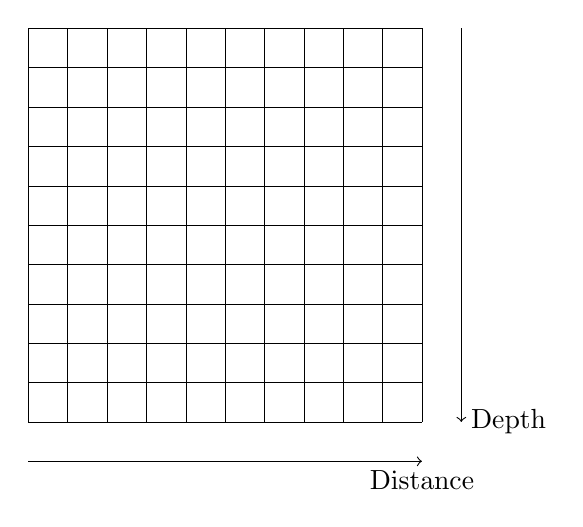
\begin{tikzpicture}
  \draw[step=0.5, line width=0.1] (0,0) grid(5.0,5.0) ; 
  \draw[->] (0.0,-0.5) -- (5.0,-0.5) node[below]{Distance};
  \draw[->] (5.5,5.0) -- (5.5,0.0) node[right]{Depth};
\end{tikzpicture}
\end{frame}
%---------------------------------------------------
\begin{frame}{Numerical engine}
%---------------------------------------------------
%
Finite-difference solution of the acoustical wave equation
\begin{eqnarray}
    \sigma(x,z,t+\Delta t)           & = &2\sigma(x,z,t) - \sigma(x,z,t-\Delta t) \nonumber\\
                       & + &\Delta t^2{\kappa(x,z)}[\d_{x} \ddot{u}_x(x+\Delta x/2,z,t)+ \nonumber \\
                       &  + &\d_{z} \ddot{u}(x,z+\Delta z/2,t)]
                         + \Delta t^2 \ddot{I}(z,t).\nonumber\\
                                                       \label{eq:ch4-506}
\end{eqnarray}
Input to RTM
\begin{enumerate}
  \item P-wave velocity model on a 3D grid covering surface area and depth range to be imaged.
        Typical values (depending on area) could be 10x20x5km. 
  \item Preprocessed shot records typical 1000000 shots.
\end{enumerate}  
%
\end{frame}
%---------------------------------------------------
\begin{frame}{Numerical engine}
%---------------------------------------------------
Key parameters to be determined
\begin{enumerate}
  \item $\Delta t$ of the data
  \item $\Delta t$ for the time stepping
  \item $\Delta x$ for the data
  \item $\Delta x$ for the grid
\end{enumerate}
The sampling interval for the data is determined by the effective frequency content.
A sampling interval of 4ms gives a nyquist frequency of
\begin{eqnarray}
f_n = 1/2\Delta t = 1/(2*0.004) = 125Hz
\end{eqnarray}
which is probably adequat for most exploration cases.
\end{frame}
%---------------------------------------------------
\begin{frame}{Numerical engine}
%---------------------------------------------------
The time stepping $\delta t$ is determined by two factors
\begin{itemize}
  \item Stability
  \item Numerical accuracy (Dispersion)
\end{itemize}
Stability is given approximately by the largest velocity
\begin{eqnarray}
c_{max} \Delta t \le 2\Delta x/\sqrt{3}
\end{eqnarray}
Dispersion is dependent on the approximation for the second order time derivative,
but a rough rule is 
\begin{eqnarray}
\frac{\lambda}{c\Delta t} \approx 10-20
\end{eqnarray}
If $\lambda$=20m and $c=$2000m/s this
implies $\Delta t < $0.001 seconds
\end{frame}
%---------------------------------------------------
\begin{frame}{Boundary conditions as source}
%---------------------------------------------------
The imaging formula is:
\begin{eqnarray}
 r(\xx',\xx,t=0)=
\int dS(\xx_s)\, \int d\tau\, p(\xx',\xx_s,\tau)\partial_z p_0(\xx,\xx_s,\tau)\nonumber\\
&&                   \label{eq:10600}
\end{eqnarray}
$p_0$ is a forward modeled wavefield which is the solution of the acoustic
wave equation
\begin{eqnarray}
\nabla^2 p(\xx,t,\xx_s) - \frac{1}{c^2(\xx)} \partial^2_t p(\xx,\xx_s,t) = \delta(\xx-\xx_s)h(t)
\end{eqnarray}
Here $c(\xx)$ is the velocity model.
\end{frame}
%---------------------------------------------------
\begin{frame}{Boundary conditions as source}
%---------------------------------------------------
$p(\xx,\xx_s,t)$ is a wavefield with time-reversed boundary conditions
\begin{eqnarray}
p(\xx,\xx_s,t) =
-\int dS(\xx')\, p(\xx',\xx_s,-t)*\partial_z' g(\xx,\xx',t)
&&                   \label{eq:1000}
\end{eqnarray}
\end{frame}
%---------------------------------------------------
\begin{frame}{Boundary conditions as source}
%---------------------------------------------------
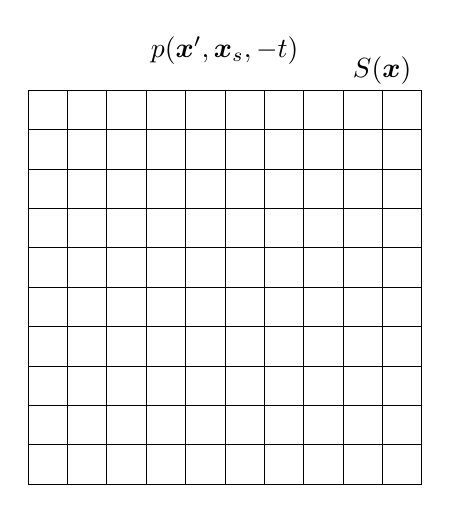
\begin{tikzpicture}
  \draw[step=0.5, line width=0.1] (0,0) grid(5.0,5.0) ; 
%  \draw[->] (-0.5,-0.5) -- (5.5,-0.5);
  \node at (2.5,5.5) {$p(\xx',\xx_s,-t)$} ;
  \node at (4.5,5.25) {$S(\xx)$} ;
\end{tikzpicture}
It is difficult to introduce the data as a pure boundary condition in 
the finite-difference method (but not impossible). Instead it is easier
to replace the boundary condition with sources.
\end{frame}
%---------------------------------------------------
\begin{frame}{Boundary conditions as source}
%---------------------------------------------------
\begin{eqnarray}
p(\xx,\xx_s,t)  = \nonumber\\
 - \int dV(\xx'')\left[\int dS(\xx')\, p(\xx',\xx_s,-t)\partial_z \delta(\xx''-\xx')\right]*g(\xx,\xx'',t)
                  \label{eq:2000}
\end{eqnarray}
%
Here we have used the fact that
\begin{eqnarray}
f'(0) = \int dx\, \partial_x \delta(x)
\end{eqnarray}
The solution of the acoustic wave equation can be written
\begin{eqnarray}
p(\xx,\xx_s,t) = \int dV(\xx'') g(\xx,\xx'',t)* s(\xx'',t)
                              \label{eq:3000}
\end{eqnarray}
Comparing equations \eqref{eq:3000} and \eqref{eq:2000} we see that the surface integral over 
the data and the derivative of the delta function is simply a source where each receiver point is
a source with strength:
\begin{eqnarray}
    p(\xx',\xx_s,-t)\partial_z \delta(\xx''-\xx').
\end{eqnarray}
\end{frame}
%---------------------------------------------------
\begin{frame}{Storage requirements}
%---------------------------------------------------
The algorithm for RTM can be summarized as:
\begin{enumerate}
  \item Forward model a single shot record with a point source
        Store wavefield for all timesteps
  \item Backward model a single shot record with the data acting as sources
        Store wavefield for all timesteps
  \item Cross-correlate (zero-time lag) the forward and backward wavefields
  \item repeat for all shots and sum over shots
\end{enumerate}
Storage is needed because the backward field is computed
in reverse time order and need to be reordered before cross-correlation
\end{frame}
%---------------------------------------------------
\begin{frame}{Storage requirements}
%---------------------------------------------------
Migration of the sigsbee 2D model (Very small example
compared to 3D industrial migrations).
\begin{figure}
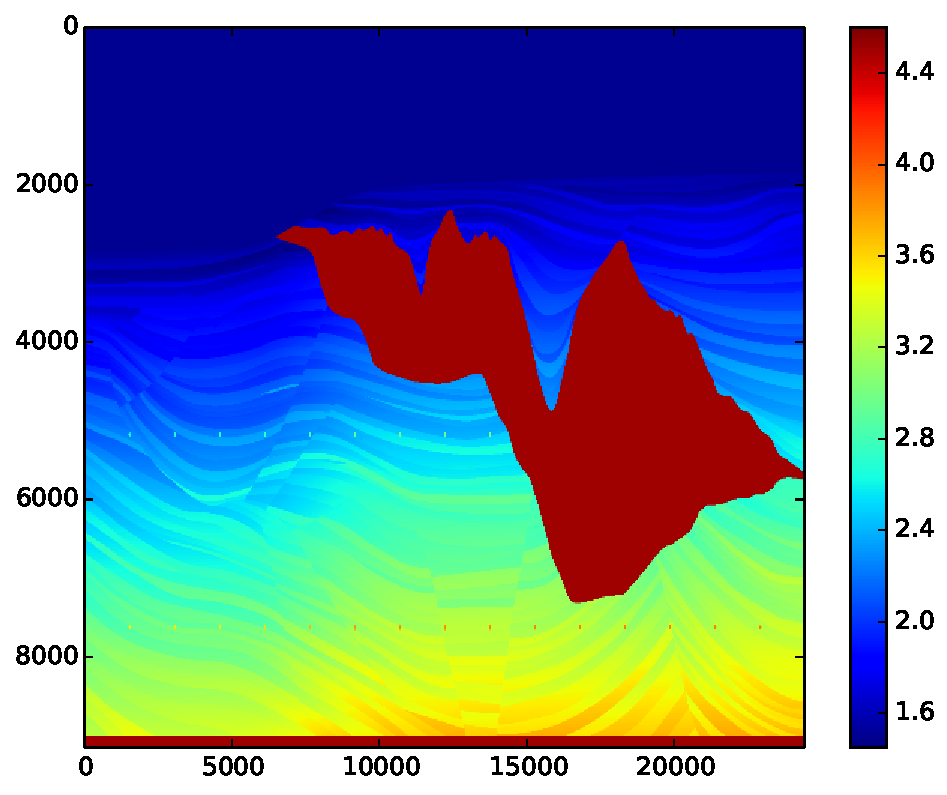
\includegraphics[width=0.75\textwidth]{Fig/vp-original.pdf}
\end{figure}
\end{frame}
%---------------------------------------------------
\begin{frame}{Storage requirements}
%---------------------------------------------------
Synthetic example with parameters
\begin{itemize}
\item No of gridpoints Nx=1496, Nz=601
\item Length of model: $\approx$ 37km
\item Depth of model:  $\approx$ 9 km
\item Grid sampling : $\Delta x \approx 15$m.
\item Time sampling : $\Delta t$ : 0.0005 sec
\item Receiver group spacing: 23m
\item Number of receiver gropups: 348
\item Streamer length: 8km
\item Shot distance: 45m
\item No of shots: 500
\item Migration aperture: 15km
\item Shot record length: 12sec
\end{itemize}
\end{frame}
%---------------------------------------------------
\begin{frame}{Storage requirements}
%---------------------------------------------------
Synthetic example with parameters
\begin{itemize}
\item Size of one snapshot: $1000 \times 600 \times 4 = 2.4 \times 10^6$
\item No of snapshots: $24000$
\item Total storage req for the forward modelled wavefield: $2.4\times 10^6\times 24000: 5.76\times 10^9 = $58Gb
\item Total storage req $\times$58Gb $\approx$ 120Gb
\item Cpu time for one shot: 30 minutes implies 10 days for 500 shots.
\item Migrate 100 shots in parallel: 2.5 Hours.
\item Storage req increase to 120Gb $\times$ 100 = 12Tb.
\end{itemize}
Storage is a problem with this approach.
\end{frame}
%---------------------------------------------------
\begin{frame}{Storage requirements}
%---------------------------------------------------
Modified storage approach
\begin{itemize}
\item Only store some snapshots, i.e every 0.005 seconds
\item Reduced storage to 1.2Tb
\item Use compression to further reduce storage
\item Interpolation is needed for high quality
\end{itemize}
\end{frame}
%---------------------------------------------------
\begin{frame}{Storage requirements}
%---------------------------------------------------
Reconstruction method
\begin{itemize}
\item Store wavefield recorded at the surface when doing forward modeling
\item Storage is reduced to small amounts of data
\item Perform backward modeling of data and forward wavefield 
\item Forward wavefield no comes out in reverse time
\item Cross-correlation can then be performed immediately
\end{itemize}
Requires 50\% more computer time, but little storage.
\end{frame}
%---------------------------------------------------
\begin{frame}{Storage requirements}
%---------------------------------------------------
\begin{figure}
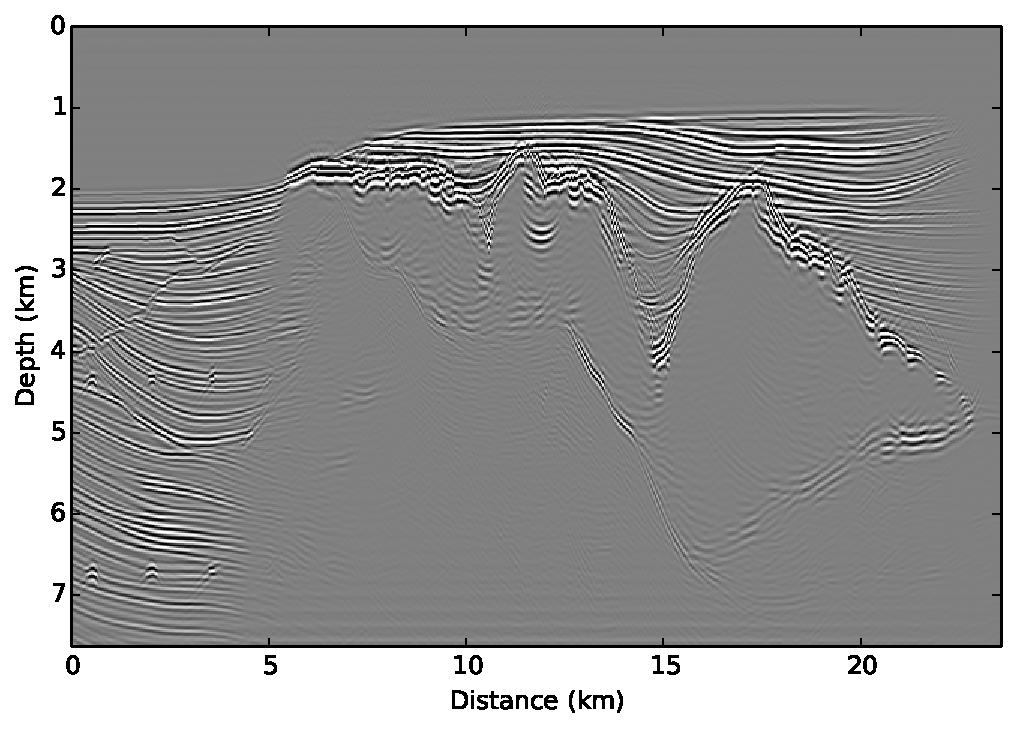
\includegraphics[width=0.9\textwidth]{Fig/mig.pdf}
\end{figure}
\end{frame}
%---------------------------------------------------
\begin{frame}{RTM Input files and parameters}
%---------------------------------------------------
\begin{itemize}
\item Shot records
\item Velocity model
\item $\Delta x$ and $\Delta t$
\item Migration aperture
\end{itemize}
Aliasing
\begin{eqnarray}
\frac{\omega}{c_{min}} \le \frac{\pi}{\Delta x} \\
f_{max} = \frac{c_{min}}{2\Delta x}\\
f_{max} = \frac{1500}{2\times 15} = 30Hz
\end{eqnarray}
\end{frame}
%---------------------------------------------------
\begin{frame}{RTM Angle gathers}
%---------------------------------------------------
In addition to the output (zero-offset) image, so-called angle
gathers contain additional information on the angle behaviour of
the reflectivity. This information is often used for identifying 
hydrocarbons or classifying rocktypes. 
\begin{figure}
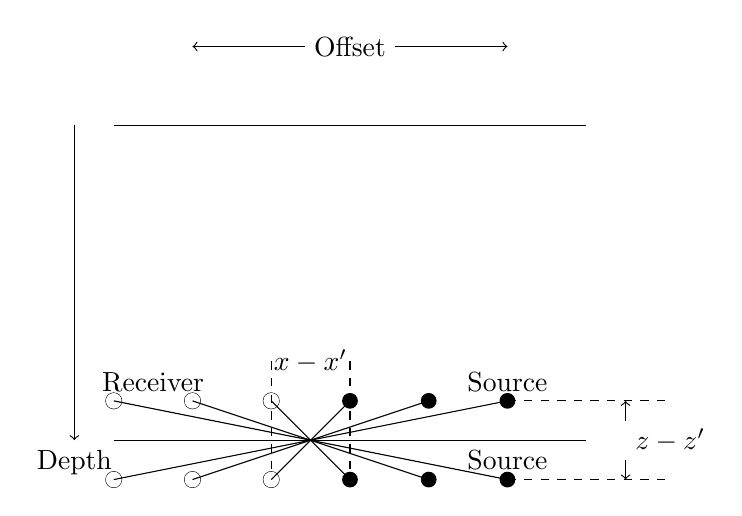
\begin{tikzpicture}[scale=1.0]
   \draw[->] (-0.5,4.0) -- (-0.5,0.0) node[below]{Depth} ;      %Depth axis 
   \draw[<->] (1.0,5.0) -- node[fill=white]{Offset} (5.0,5.0);  %Offset axis  
  \draw (0.0,4.0) -- (6.0,4.0) ;                               % Boundary at top
  \draw (0.0,0.0) -- (6.0,0.0) ;                               % Boundary at depth

  \fill (3.0,0.5) node[above]{} circle (0.1) ;           % Draw source
  \fill (4.0,0.5) node[above]{} circle (0.1) ;           % Draw source
  \fill (5.0,0.5) node[above]{Source} circle (0.1) ;     % Draw source text

  \draw (2.0,0.5) circle (0.1) ;             %Draw receiver
  \fill[white] (2.0,0.5) circle (0.1) ;

  \draw (1.0,0.5) circle (0.1) ;             %Draw receiver
  \fill[white] (1.0,0.5) circle (0.1) ;

  \draw (0.0,0.5) circle (0.1) ;             %Draw receiver
  \fill[white] (0.0,0.5) circle (0.1) ;
  \draw (0.5,0.5) node[above]{Receiver} ;    %Draw receiver text 

  \draw (3.0,0.5) -- (2.5,0.0);              % Draw ray from source to midpoint
  \draw (4.0,0.5) -- (2.5,0.0);              % Draw ray from source to midpoint
  \draw (5.0,0.5) -- (2.5,0.0);              % Draw ray from source to midpoint

  \draw (2.0,0.5) -- (2.5,0.0);              % Draw ray from receiver to midpoint
  \draw (1.0,0.5) -- (2.5,0.0);              % Draw ray from receiver to midpoint
  \draw (0.0,0.5) -- (2.5,0.0);              % Draw ray from receiver to midpoint

  \draw[dashed] (2.0,1.0) -- (2.0,-0.5);     %Draw vertical dashed line
  \draw[dashed] (3.0,1.0) -- (3.0,-0.5);     %Draw vertical dashed line
  \draw (2.5,1.0) node {$x-x'$};           % Draw equation
  \draw[dashed] (5.0,0.5) -- (7.0,0.5);     %Draw vertical dashed line
  \draw[dashed] (5.0,-0.5) -- (7.0,-0.5);     %Draw vertical dashed line
  \draw (6.5,0.0) node[right]{$z-z'$};           % Draw equation
  \draw[->] (6.5,0.25) -- (6.5,0.5);
  \draw[->] (6.5,-0.25) -- (6.5,-0.5);



  \fill (3.0,-0.5) node[above]{} circle (0.1) ;           % Draw source
  \fill (4.0,-0.5) node[above]{} circle (0.1) ;           % Draw source
  \fill (5.0,-0.5) node[above]{Source} circle (0.1) ;     % Draw source text

  \draw (2.0,-0.5) circle (0.1) ;             %Draw receiver
  \fill[white] (2.0,-0.5) circle (0.1) ;

  \draw (1.0,-0.5) circle (0.1) ;             %Draw receiver
  \fill[white] (1.0,-0.5) circle (0.1) ;

  \draw (0.0,-0.5) circle (0.1) ;             %Draw receiver
  \fill[white] (0.0,-0.5) circle (0.1) ;
  %\draw (0.5,0.5) node[above]{Receiver} ;    %Draw receiver text 

  \draw (3.0,-0.5) -- (2.5,0.0);              % Draw ray from source to midpoint
  \draw (4.0,-0.5) -- (2.5,0.0);              % Draw ray from source to midpoint
  \draw (5.0,-0.5) -- (2.5,0.0);              % Draw ray from source to midpoint

  \draw (2.0,-0.5) -- (2.5,0.0);              % Draw ray from receiver to midpoint
  \draw (1.0,-0.5) -- (2.5,0.0);              % Draw ray from receiver to midpoint
  \draw (0.0,-0.5) -- (2.5,0.0);              % Draw ray from receiver to midpoint
\end{tikzpicture}
\end{figure}
\end{frame}
%---------------------------------------------------
\begin{frame}{RTM Angle gathers}
%---------------------------------------------------
Use the offset and time delay formula
\begin{eqnarray}
 r(\xx',\xx,t)=r(\xx'=0,\xx,\nonumber\\
\int dS(\xx_s)\, \int d\tau\, p(\xx',\xx_s,\tau+t)\partial_z p_0(\xx,\xx_s,\tau)
&&                   \label{eq:10500}
\end{eqnarray}
We want to compute the plane-wave reflectivity. The simplest way is to use the so-called $\tau-p$ transform,
which is a decomposition into plane waves.
\begin{eqnarray}
r(p,\tau) = \int dx\, r(x,\tau+px)
\end{eqnarray}
\end{frame}
%---------------------------------------------------
\begin{frame}{RTM Angle gathers}
%---------------------------------------------------
\begin{figure}
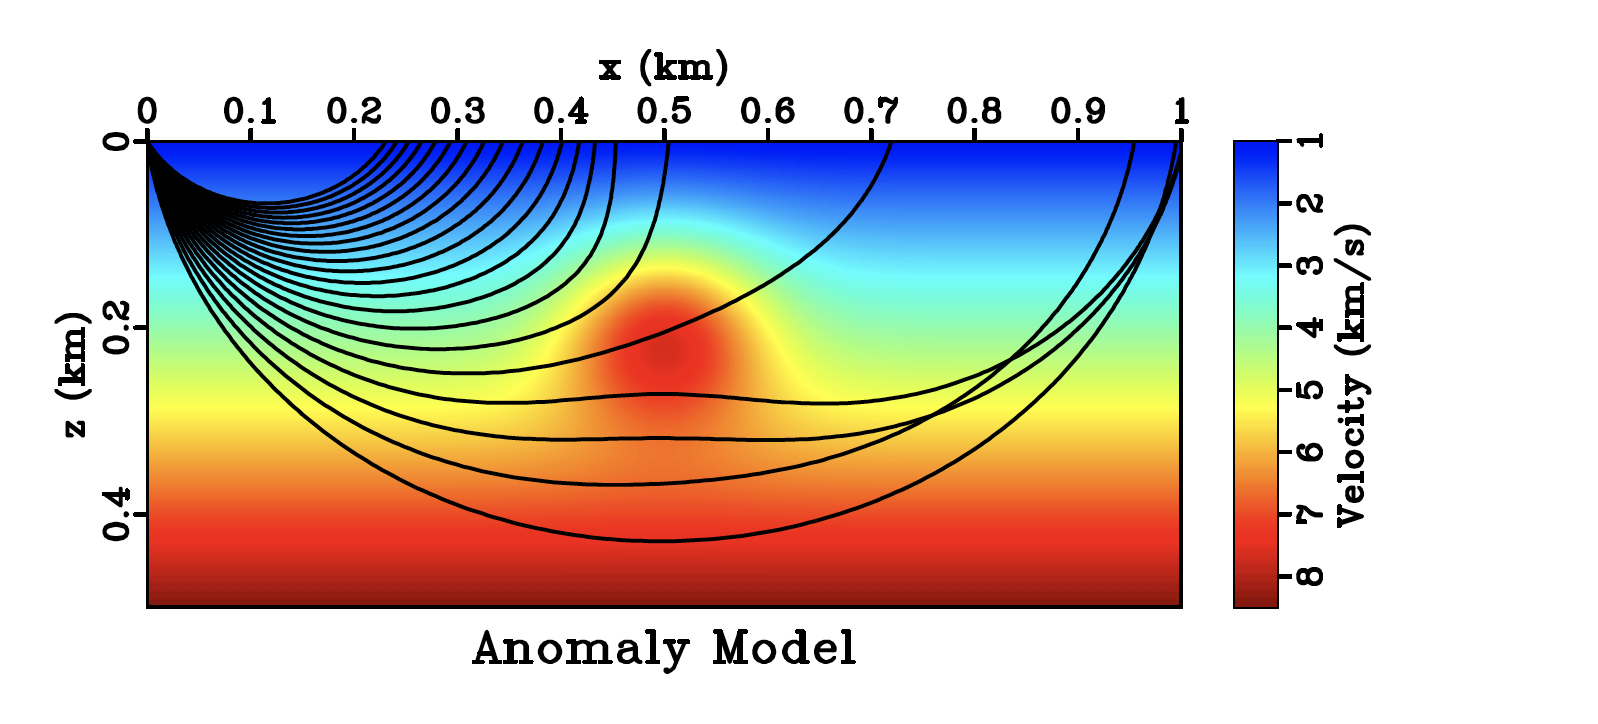
\includegraphics[width=0.5\textwidth]{Fig/fig1.pdf}
\end{figure}
\end{frame}
%---------------------------------------------------
\begin{frame}{RTM Angle gathers}
%---------------------------------------------------
\begin{figure}
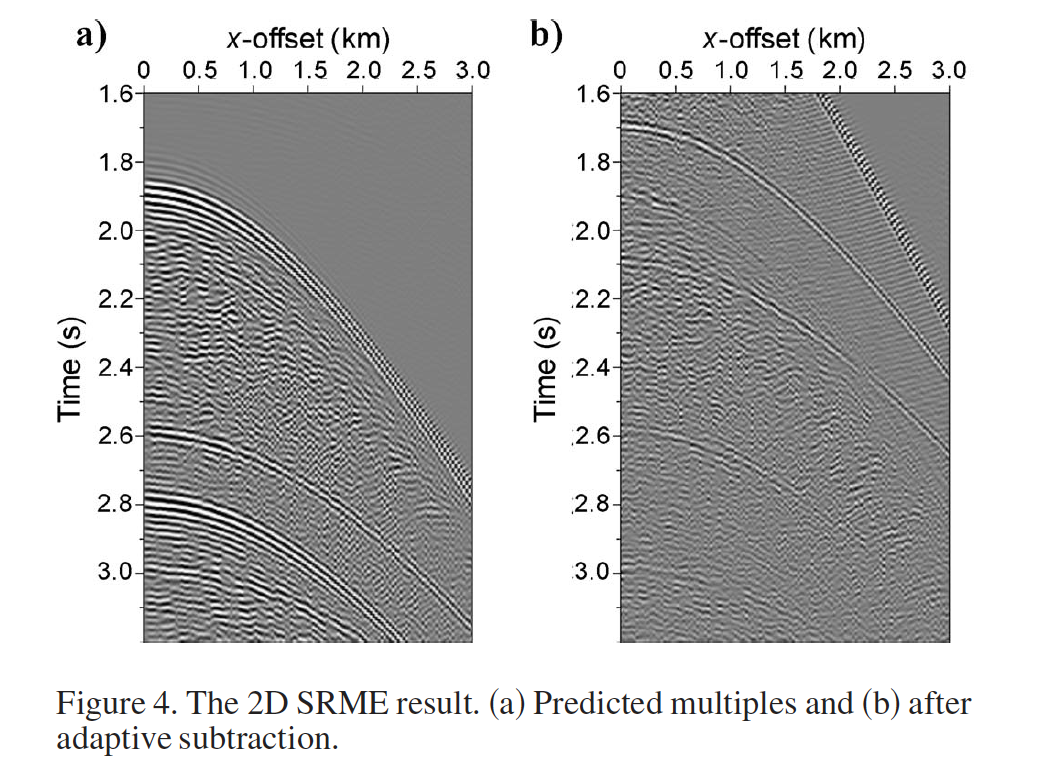
\includegraphics[width=\textwidth]{Fig/fig2.pdf}
\end{figure}
\end{frame}
%---------------------------------------------------
\begin{frame}{RTM Angle gathers}
%---------------------------------------------------
\begin{figure}
\includegraphics[width=\textwidth]{Fig/fig11.pdf}
\end{figure}
\end{frame}
%---------------------------------------------------
\begin{frame}{RTM Angle gathers}
%---------------------------------------------------
\begin{figure}
\includegraphics[width=\textwidth]{Fig/fig12.pdf}
\end{figure}
\end{frame}
%---------------------------------------------------
\begin{frame}{RTM Angle gathers}
%---------------------------------------------------
\begin{figure}
\includegraphics[width=\textwidth]{Fig/fig13.pdf}
\end{figure}
\end{frame}
%---------------------------------------------------
\begin{frame}{RTM Angle gathers}
%---------------------------------------------------
\begin{figure}
\includegraphics[width=0.4\textwidth]{Fig/fig14.pdf}
\end{figure}
\end{frame}
%---------------------------------------------------
\begin{frame}{RTM Angle gathers}
%---------------------------------------------------
\begin{figure}
\includegraphics[width=0.9\textwidth]{Fig/fig15.pdf}
\end{figure}
\end{frame}
\end{document}
